\section{Measurements and Results}
\label{sec:Measurements}
A test sample base was created with ten tracks for each class. All of the test samples were new samples that were not included in the training sample base.

\subsection{Modified Mini Batch $k$-Means}
The $k$-Means algorithm was used to calculate $k=10$ class centers in our sample base using a batch size of 500 points and 50 iterations. These classes were used to classify our test sample base. The tags of the test samples within each of the 10 class clusters created by the $k$-Means algorithm were counted. The results are shown in figure~\ref{fig:k-Means}.\\
It can be seen that the algorithmically calculated classes do not correspond well to the tags defined by our sample base. In eight different measurements the percentage of right classified samples was 23~\% in the mean, minimum 8.3~\% and maximum 33.3~\%. Such modest results were to be expected. Nevertheless, it seems that there are some consistent mappings in the structuring of the tags. This needs to be verified with further research. % 28, 30, 34, 40, 10, 10, 37, 34 of 120
\begin{figure}[htbp]
\centering
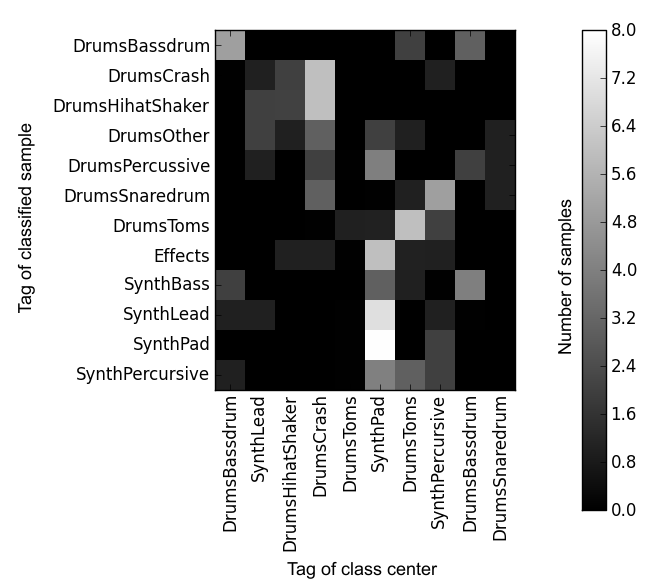
\includegraphics[width=0.45\linewidth]{../measurements/k_means_1_mod.png}
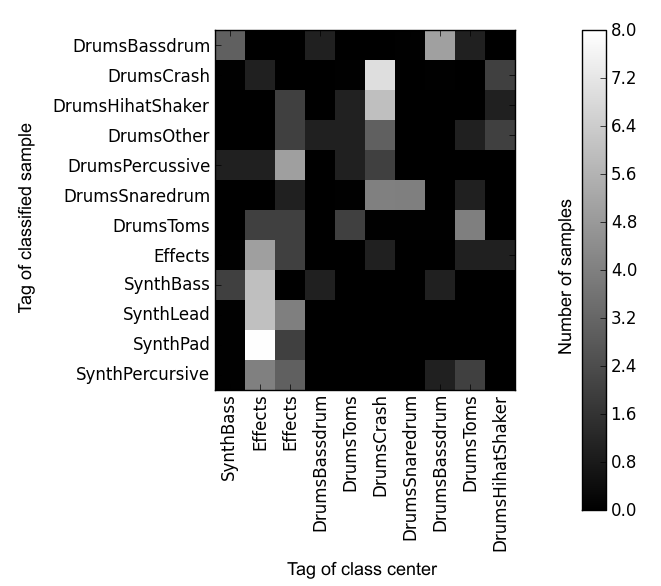
\includegraphics[width=0.45\linewidth]{../measurements/k_means_2_mod.png}
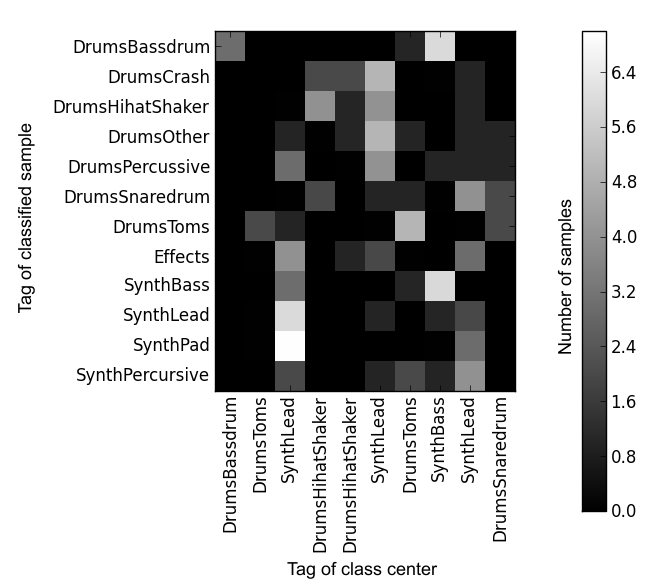
\includegraphics[width=0.45\linewidth]{../measurements/k_means_3_mod.png}
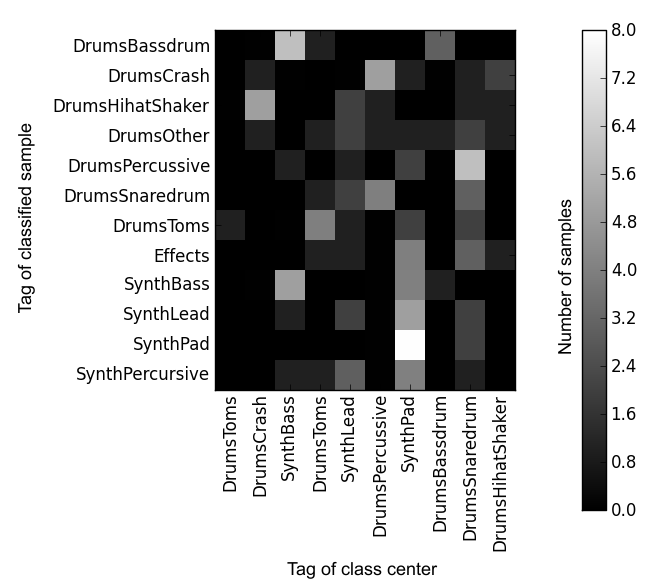
\includegraphics[width=0.45\linewidth]{../measurements/k_means_4_mod.png}
\caption{Number of samples, depending on their tag and the tag of the class center they were assigned to. The 10 classes were generated by a modified mini batch $k$-Means algorithm with a batch size of 500 using 50 iterations. The four plots represent four different runs of the modified mini batch $k$-Means algorithm.}
\label{fig:k-Means}
\end{figure}

\subsection{$k$-Nearest-Neighbors}
All the samples in the test sample bank were classified using the implemented $k$-NN algorithm with $k=10$. The results are shown in figure~\ref{fig:k-NN}. The tags of the test bank are plotted against the tags of the classification.\\
The results show that many of the samples are classified correctly. The percentage of correct classified samples is 48.3~\%. This even exceeds our expectations. The variations in the classification correlate with the variances between samples of the same tag in the sample base. This means that the classes that are badly classified are also hard to classify by human perception.
%right class hits:  58
%wrong class hits:  62
%percentage right:  48.333333333333336

\begin{figure}[htbp]
\centering
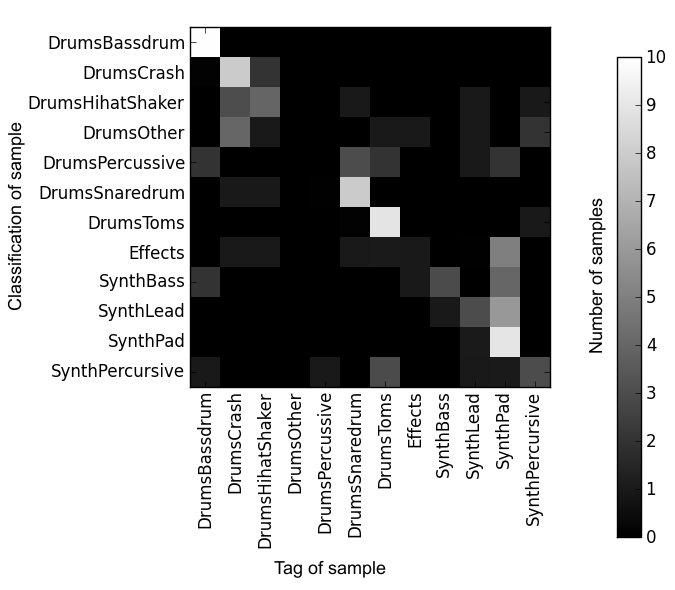
\includegraphics[width=0.47\linewidth]{../measurements/knn_mod.png}
\caption{Number of Samples, depending on their tag and the assigned tag by the $k$-NN algorithm with $k=10$.}
\label{fig:k-NN}
\end{figure}
